
We developed a compiler that compiles LM programs to byte-code and a multi-threaded
virtual machine (VM) using the Pthreads library to run the byte-code.
The goal of our system is to keep the threads as busy as possible and to reduce inter-thread communication.

The load balancing aspect of the system is performed by our work scheduler that is based on a work
stealing algorithm. Initially, the system will partition the application
graph of $N$ nodes into $P$ subgraphs (the number of threads) and then each thread will work on their own subgraph.
During execution, threads can steal nodes of other threads to keep themselves busy.

Reduction of inter-thread communication is achieved by first ordering the node addresses present
in the code in such a way that closer nodes are clustered together and then partitioning them
to threads. During compilation, we take note of predicates that are used in rules for
communication rules (arguments with type \emph{node}) and then build a graph of nodes from
the program's axioms. The nodes of the graph are then ordered by using a breadth-first search
algorithm that changes the nodes of addresses to the domain $[0, n[$, where $n$ is the number of
nodes. Once the VM starts, we simply partition the range
$[0, n[$.

\subsection{Threads}

When the VM starts, it reads the byte-code file and starts all threads.
The partitioning of nodes is performed by dividing the domain of node addresses across the number of available threads.
In Fig.~\ref{fig:overview} we present the overview of a virtual machine running 2 threads and a program with 6 nodes.
Node that the dotted arrows represent the edges between nodes. In each thread space, we place the nodes owned by each thread.
Initially, the threads grab their own nodes and assign the \texttt{owner} property of each.
Because only one thread is allowed to do computation on a node at any giving time, the owner property
defines the thread with such permission.

\begin{figure*}[ht]
   \centering
   \scalebox{0.60}{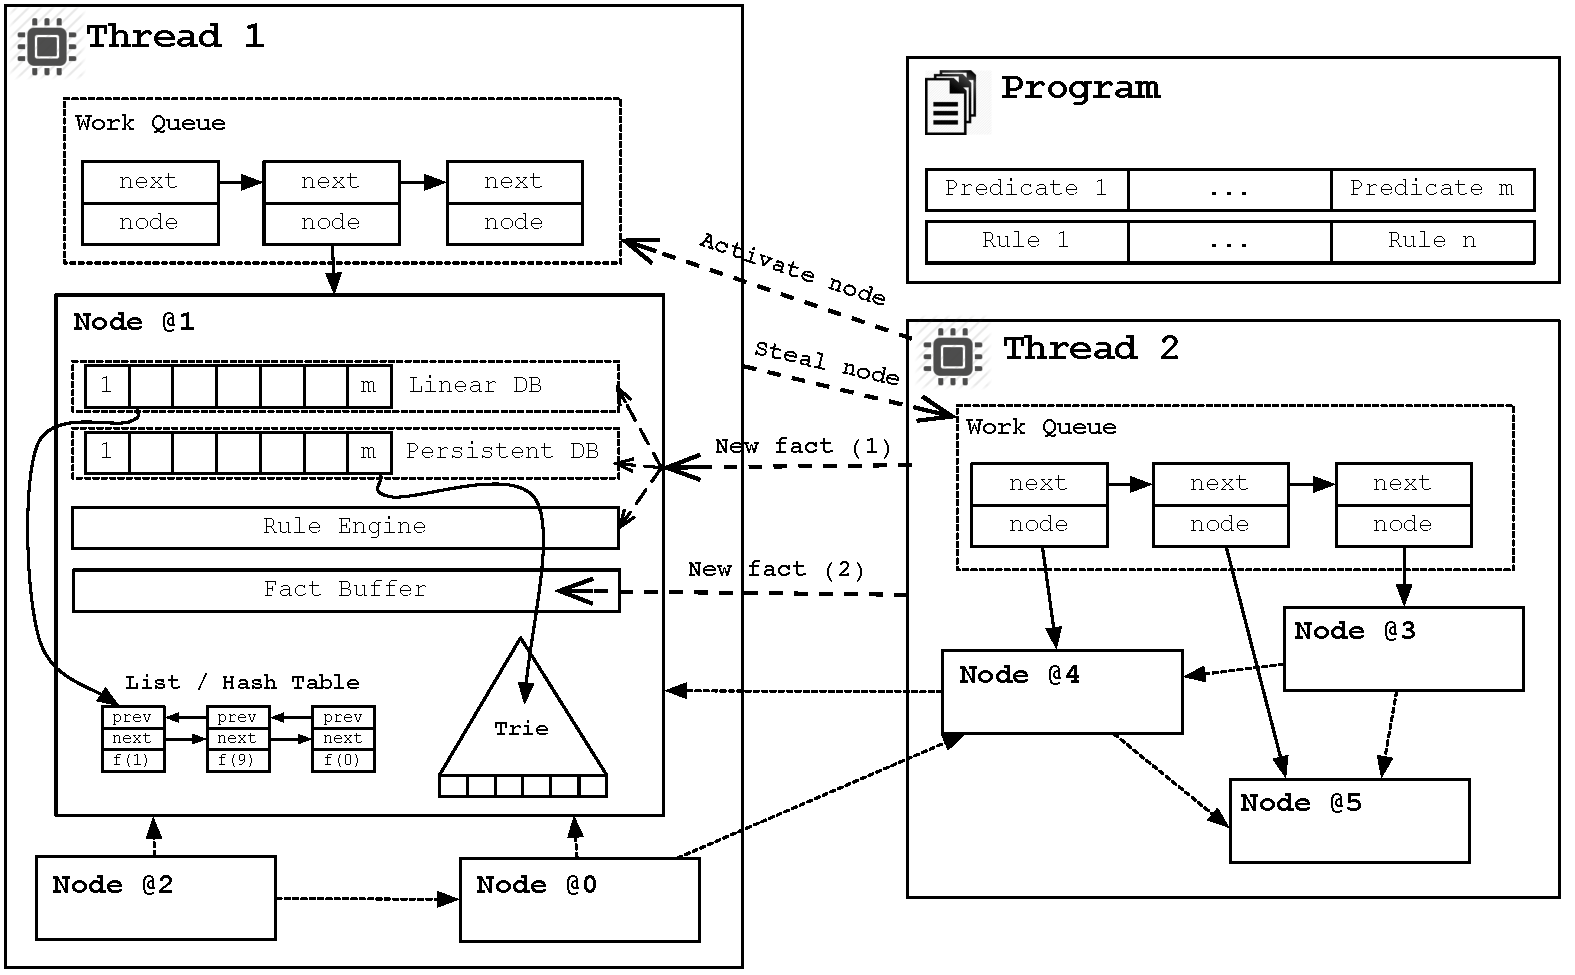
\includegraphics[]{overview.pdf}}
   \caption{Overview of the virtual machine (showing 2 threads).}
   \label{fig:overview}
\end{figure*}

Included in the thread space is the \emph{Work Queue}, a single linked list containing \emph{active nodes}, i.e.,
nodes that have new facts to process. Initially, the \emph{Work Queue} is filled with all the nodes of the thread
in order to derive the axioms.

The main thread loop is shown in Fig.~\ref{code:work_loop}, where the threads
inspects their work queue for active nodes. Procedure \texttt{process\_node()} takes a node with new candidate rules
and executes them. If the work queue is empty, the thread attempts to steal one node from another thread before
becoming idle (\emph{Steal node} in Fig.~\ref{fig:overview}). Starting from a random thread, it cycles through all the threads to find one active node.
Eventually, there will be no more work to do and the threads will go idle. There is a global atomic counter, a global
boolean flag and one boolean flag for each thread that are used to detect termination.
Once a thread goes idle, it decrements the global counter and changes its flag to idle. If the counter
reaches zero, the global flag is set to idle. Since every thread will be busy-waiting and checking
the global flag, they will detect the change and stop executing.

\begin{figure}[h!]
\scriptsize\begin{Verbatim}
void work_loop(thread_id tid):
   while (true):
      current_node = NULL;
      if(has_work(tid)):
         current_node = pop_work(tid); // take node from the queue
      else:
         target_thread = random(NUM_THREADS);
         for (i = 0; i < NUM_THREADS && current_node == NULL; ++i):
            // need to steal a node
            target_thread = (target_thread + 1) % NUM_THREADS;
            current_node = steal_node_from_thread(target_thread)
      if(current_node == NULL):
         become_idle(tid);
         if(!synchronize_termination(tid)):
            return;
         become_active(tid);
      else:
         process_node(current_node, tid);
\end{Verbatim}
  \caption{Thread work loop.}
  \label{code:work_loop}
\end{figure}

\subsection{Nodes}

In Fig.~\ref{fig:overview}, we also present the internal structure of a node (node \texttt{@1}). Each node
contains the following: a database composed of \emph{Linear DB} (linear facts) and \emph{Persistent DB} (persistent facts) (further explained in \ref{sec:database});
rule matching structures (\emph{Rule Matching Structures}); and a \emph{Fact Buffer}, for storing intermediate facts coming
from other threads.

Whenever a new fact is derived through rule derivation, we need to update the data structures for the corresponding node.
This is trivial if the thread that owns the node derived the fact also. However, if that is not the case, then we have to synchronize
since multiple threads need to update the same data structures. We added a lock and a boolean flag to each node to protect the access to its data structures.
For example, in Fig.~\ref{fig:overview}, if thread 2 derives a fact to node \texttt{@1} (owned by thread 1), then thread 2 checks the node's flag
and if not activated, will lock node \texttt{@1} and then perform the required updates (\emph{New fact (1)}). If the flag is activated, it means
that thread 1 is currently executing the node, therefore it will not touch the main node data structures, but instead will add the new fact
to \emph{Fact Buffer} (\emph{New fact (2)}). The facts stored in \emph{Fact Buffer} will then be processed by thread 1 whenever the node is about to be executed.

Another thread interaction happens during fact derivation. In the example, after the fact is derived and sent to node \texttt{@1}, thread 2 also may need
to activate node \texttt{@1} by pushing it to the \emph{Work Queue} of thread 1 (\emph{Activate node}). Each node has another flag called \emph{In Queue} that indicates
if the node is currently placed in the \emph{Work Queue}. If the node is not in the queue, then we push it to the queue and then check if the target thread is currently idle.
After this synchronization point, the target thread will be active and with a new node to process.

\subsubsection{Database Data Structures}\label{sec:database}

We said before that LM rules are constrained by the first argument. Because nodes can execute
independently, our database is indexed by the node address and each sub-database does not
need to deal with synchronization issues since at any given point, only one thread will be using
the database. Note that the first argument of each fact is not stored.

The database must be implemented efficiently because during matching of rules we need
to restrict the facts using a given \emph{match object}, which fixes arguments of the target predicate to instantiated values.
Each sub-database is implemented using three kinds of data structures:

\begin{itemize}
   \item \emph{Trie Data Structures} are used exclusively to store persistent facts.
   Tries are trees where facts are indexed by the common arguments.
      
   \item \emph{Doubly Linked List Data Structures} are used to store linear facts.
   We use a double linked list because it is very efficient to add and remove facts.
   
   \item \emph{Hash Table Data Structures} are used to improve lookup when linked lists are too long and when we need to do search filtered by a fixed argument. The virtual machine decides which arguments are best to be indexed
   (see "Indexing") and then
   uses an hash table indexed by the appropriate argument. If we need to go through all the facts, we just iterate through all the facts in the table. For collisions, we use the above doubly linked list data structure.
\end{itemize}

\begin{figure}[]
   \centering
   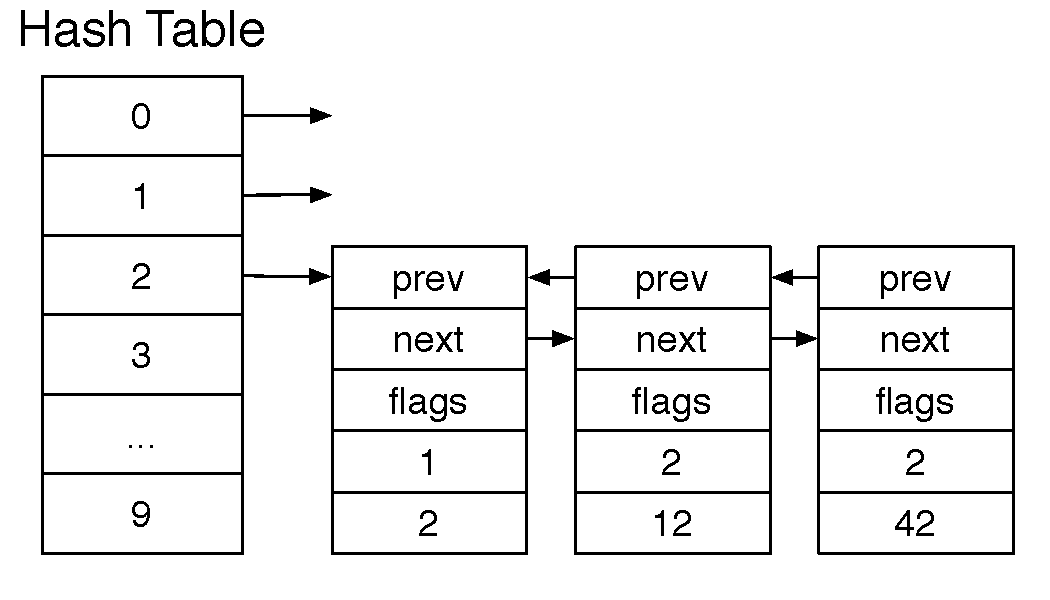
\includegraphics[width=0.40\textwidth]{hash_table.pdf}
   \caption{\small{Hash table data structure for storing predicate \texttt{a(int,int)}.}}
   \label{fig:hash_table}
\end{figure}

Figure~\ref{fig:hash_table} shows an example for a hash table data structure
with 3 linear facts indexed by the second argument and stored as doubly linked list
in bucket \texttt{2}. Each linear fact contains the regular list pointers, a \texttt{flags} field
and the fact arguments. Those are all stored continuously to improve data
locality. One use of the \texttt{flags} field is to mark that a fact is already being used. For example,
consider the rule body \texttt{a(A,B), a(C,D) -o ...}. When we first pick a fact for \texttt{a(A, B)} from the hash table,
we mark it as being used in order to ensure that, when we retrieve facts for \texttt{a(C, D)}, the first one
cannot be used since that would violate linearity.

\subsubsection{Rule Engine}\label{rule_engine}

The rule engine decides which rules may need to be executed while taking into account rule priorities.
There are 5 main data structures for scheduling rule execution;
\texttt{Rule Queue} is the bitmap representing the rules that will be run;
\texttt{Active Bitmap} contains the rules that have enough facts to be fired;
\texttt{Inactive Bitmap} contains the rules that must be dropped from \texttt{Rule Queue};
\texttt{Predicates Bitmap} marks the newly derived facts;
and \texttt{Predicates Count} counts the number of facts per predicate.
To understand how our engine works, consider the following rules and axioms:

{\footnotesize\begin{Verbatim}
// rules
a, e(1) -o b.
a -o c.
b -o d.
e(0) -o f.
c -o e(1).

// axioms
a.
e(0).
\end{Verbatim}
}

\begin{figure*}[]
   \centering
   \scalebox{0.7}{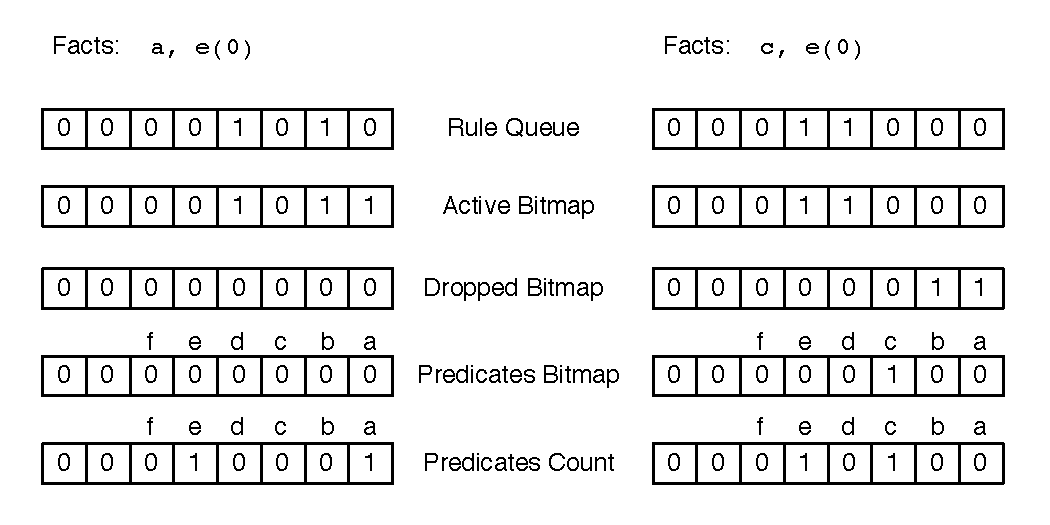
\includegraphics[]{rule_queue1.pdf}}
   \caption{Program and rule engine data structures: before and after applying the \nth{2} rule.}
   \label{fig:rule_engine}
\end{figure*}


In our example, since we have facts \texttt{a} and \texttt{e(0)},
we will execute the second rule \texttt{a -o c}.
In order to pick such rule, we need to take the least significant bit from the \texttt{Rule Queue} bitmap.
Because the derivation is successful, we will consume \texttt{a} and derive \texttt{c}.
We thus mark the \texttt{c} predicate in the \texttt{Predicates Bitmap} and the first and second rules
in \texttt{Dropped Bitmap} since such rules are no longer applicable (\texttt{a} is gone). To update the \texttt{Rule Queue},
we remove the bits marked in \texttt{Dropped Bitmap} and add the active rules marked in \texttt{Active Bitmap} that are affected
by predicates in \texttt{Predicates Map}. The engine thus schedules the fourth and fifth rules to run (Fig.~\ref{fig:rule_engine}b).

Note that every node in the program has the same set of data structures present in Fig.~\ref{fig:rule_engine}.
We use 32 bits integers to implement bitmaps and an array of 16 bits integers to count facts, resulting in
$32 + 2P$ bytes per node, where $P$ is the number of predicates.

We do a small optimization to reduce the number of derivations of persistent facts. We
divide the program rules into two sets: \emph{persistent rules} and \emph{non persistent rules}.
Persistent rules are rules where only persistent facts are involved. We compile such rules
incrementally, that is, we attempt to fire all rules where a persistent fact is used. This is called
the \emph{pipelined semi-naive} evaluation and it originated in the P2 system~\cite{Loo-condie-garofalakis-p2}.
This evaluation method avoids excessing re-derivations of the same fact. The order of derivation does not matter for those rules, since
only persistent facts are used.

\subsection{Byte-Code}

A byte-code file contains meta-data about the program's predicates, initial nodes, partitioning
information, and code for each rule.
Each VM thread has 32 registers that are used during rule execution.
Registers can store facts, integers, floats, node addresses and pointers to runtime 
data structures (lists and structures). When registers store facts, we can reference
fields in the fact through the register.

Consider a rule \texttt{!a(X,Y), b(X,Z), c(X,Y) -o d(Y)} and a database with
\texttt{!a(1,2)}, \texttt{!a(2,3)}, \texttt{b(1,3)}, \texttt{b(5,3)}, \texttt{c(1,2)}, \texttt{c(1,3)},
\texttt{c(5,3)}. Rule execution proceeds in a series of recursive loops, as follows: the first loop retrieves an
iterator for the persistent facts of \texttt{!a/2} and moves the first valid fact, \texttt{!a(1,2)},
to register 0; the inner loop retrieves linear facts that match \texttt{b(1,Z)} (from the
\emph{join constraint}) and moves \texttt{b(1,3)} to register 1; in the final
loop we move \texttt{c(1,2)} to register 2 and the body of the rule is successfully matched. Next, we
derive \texttt{d(2)}, where \texttt{2} comes from register 0.
Fig.~\ref{fig:byte_code} shows the byte-code for this example.

\begin{figure}[]
\scriptsize\begin{Verbatim}
PERSISTENT ITERATE a MATCHING TO reg 0
  LINEAR ITERATE b MATCHING TO reg 1
      (match).0=0.0
    LINEAR ITERATE c MATCHING TO reg 2
        (match).0=0.0
        (match).1=0.1
      ALLOC d TO reg 3
      MVFIELDFIELD 0.1 TO 3.0
      ADDLINEAR reg 3
      REMOVE reg 2
      REMOVE reg 1
      TRY NEXT
    NEXT
  NEXT
RETURN
\end{Verbatim}
\caption{\small{Byte-code for rule \texttt{!a(X,Y), b(X,Z), c(X,Y) -o d(Y).}}}
\label{fig:byte_code}
\end{figure}

In case of failure, we jump to the previous outer loop in order to try the next candidate fact.
If a rule matches and the head is derived, we backtrack to the inner most \emph{valid loop}, i.e.,
the first inner loop that uses linear facts or, if there are no linear facts involved, to the previous 
inner loop. We need to jump to a valid loop because we may have loops with linear facts that are now invalid.
In our example, we would jump to the
loop of \texttt{b(X,Z)} and not \texttt{c(X,Y)}, since \texttt{b(1,3)} was consumed.

\begin{figure}[]
\scriptsize\begin{Verbatim}
LINEAR ITERATE a MATCHING TO reg 0
  MVFIELDREG 0.0 TO reg 1
  MVINTREG INT 1 TO reg 2
  reg 1 INT PLUS reg 2 TO reg 3
  MVREGFIELD reg 3 TO 0.0
  UPDATE reg 0
  TRY NEXT
RETURN
\end{Verbatim}
\caption{\small{Byte-code for rule \texttt{a(N) -o a(N+1)}.}}
\label{code:update}
\end{figure}

The compiler re-orders the fact expressions used in the body in order to make execution more
efficient. For example, it forces the join constraints in rules to appear at the beginning so
that matching will fail sooner rather than later. It also does the same for constraints.
Note that for every loop, the compiler adds the \emph{match object}, which contains information
about which arguments need to match, so that runtime matching is efficient.

Our compiler also detects cases where we re-derive a linear fact with new arguments.
For example, as shown in Fig.~\ref{code:update}, the rule \texttt{a(N) -o a(N+1)}
will compile to code that reuses the old \texttt{a(N)} fact.
We use a \texttt{flags} field to mark updated nodes (presented next).

\subsection{Indexing}\label{indexing}

To improve fact lookup,
the VM employs a fully dynamic mechanism to decide which argument may be optimal to index.
The algorithm is performed in the beginning of the execution and empirically tries to assess the argument
of each predicate that more equally spreads the database across the values of the argument.
A single thread performs the algorithm for all predicates.

The indexing algorithm is performed in three main steps. First, it gathers statistics of lookup data by keeping a counter
for each predicate's argument.
Every time a fact search is performed where arguments are fixed to a value, the counter of such arguments is incremented. This phase is performed during rule execution for a small fraction of the nodes in the program.

The second step of the algorithm then decides the candidate arguments of each predicate.
If a predicate was not searched with any fixed arguments, then it will be not indexed.
If only one argument was fixed, then such argument is set as the indexing argument. Otherwise, the top 2 arguments
are selected for the third phase, where \emph{entropy statistics} are collected dynamically.

During the third phase, each candidate argument has an entropy score.
Before a node is executed, the facts of the target predicate
are used in the following formula applied for the two arguments:

{\scriptsize
\[
Entropy(A, F) = - \sum_{v \in values(F, A)} \frac{count(F, A = v)}{total(F)} 	\log_2 \frac{count(F, A = v)}{total(F)}
\]
}

Where $A$ is the target argument, $F$ is the multi-set of linear facts for the target predicate, $values(F, A)$ is set of values of the argument $A$, $count(F, A = v)$ counts the number
of linear facts where argument $A$ is equal to $v$ and $total(F)$ counts the number of linear facts in $F$.
The entropy value is a good metric because it tells us how much information is needed to describe an argument.
If more information is needed, then that must be the best argument to index.

For one of the arguments to score, $Entropy(A, F)$ multiplied by the number of times it has been used for lookup must be larger than the other argument.

The argument with the best score is selected and then
a global variable called \texttt{indexing\_epoch} is updated.
In order to convert the node's linked lists into hash tables, each node also has a local variable called \texttt{indexing\_epoch}
that is compared to the global variable in order to rebuild the node database according to the new indexing
information.

Our VM also dynamically resizes the hash table if necessary. When the hash table becomes
too dense, it is resized to the double. When it becomes too sparse, it is reduced in half
or simply transformed back into a doubly linked list. This is done once in a while, before a node executes.

We have seen very good results with this scheme. For example, for the all-pairs shortest paths program,
we obtained a 2 to 5-fold improvement in sequential execution time.
The overhead of dynamic indexing is negligible since programs run almost as fast
as if the indices have been added from the start.

\subsection{Runtime Data Structures}

LM supports recursive types such as lists and pairs. These complex data structures are stored in
the heap of the VM and are managed through reference counting. For instance, each list
is a \emph{cons cell} with 3 fields: \texttt{tail}, the pointer to the next element of the list;
\texttt{head}, the element stored by this element of the list; and \texttt{refs} that counts the
number of pointers to this list element in the VM. The list is deleted from the heap whenever
\texttt{refs} is decremented to 0.
